% !TeX program = xelatex
\documentclass{assignment}
\usepackage{cite}
\usepackage{tikz}
\usetikzlibrary{arrows.meta,positioning}
\graphicspath{{../Assignment_Report_v2/figures/}{../Assignment_Report/figures/}}
\geometry{a4paper}
\hypersetup{pdftitle={Conditional Solubility Prediction for Unseen Parent Compounds},pdfauthor={COMP6133 Course Project}}

\title{Conditional Solubility Prediction for Unseen Parent Compounds\\A Study of the SOLAR-H and ExtraTrees--TabPFN Models}
\author{COMP6133 Machine Learning Course Project}
\date{18 November 2026}
\begin{document}
\maketitle
\setcounter{tocdepth}{2}
\tableofcontents
\clearpage
\section*{Abstract}
Predicting the solubility of drug molecules that never occur in the training set, across many solvents and over a span of temperatures, is a central problem in pharmaceutical processing and high-throughput screening, yet it is hampered by long-tailed sampling and cross-record leakage. Under a nested five-fold validation scheme that groups records strictly by parent scaffold, this work introduces SOLAR-H, a physics-informed structure--temperature decomposition model, together with ExtraTrees--TabPFN, a heterogeneous ensemble that couples 869 explicit intermolecular-interaction features with parent-equal weighting. ExtraTrees--TabPFN reaches the best overall results, with a parent-weighted MAE of 0.6668, an RMSE of 0.8842, and an $R^2$ of 0.5234, reducing the error of a conventional tree baseline by 8.54\%. Attribution and causal analyses confirm that the explicit interaction features dominate the predictions, and a within-combination fixed-effects treatment resolves the Simpson's paradox underlying the negative temperature correlation. The resulting system has been deployed and provides zero-error real-time inference.

\noindent\textbf{Keywords}\quad conditional solubility; unseen parents; ExtraTrees; TabPFN; SOLAR-H; parent-grouped nested validation

\section{Introduction}

\subsection{Background and Motivation}

Solubility, whether in water or in organic media, is a physicochemical property relevant to medicinal chemistry, pharmaceutics, and chemical-process engineering. During early discovery and developability assessment, more than 40\% of candidate active pharmaceutical ingredients (APIs) show restricted absorption and poor bioavailability because their solid--liquid solubility is too low, which directly curtails their viability for clinical development\cite{delaney2004,solubility2024}. Downstream, in recrystallisation purification, solvent-system selection, and liquid-formulation design, the continuous solubility behaviour of a target molecule across many industrial solvents and operating temperatures governs supersaturation control, product yield, polymorphic purity, and the attainable processing window\cite{vermeire2022,fastsolv2025}.

Faced with the vast condition space formed by a flood of novel drug scaffolds, dozens of common organic solvents, and a continuous temperature gradient, conventional trial-and-error measurements consume scarce starting materials and synthesis time, and they cannot offer full coverage once the space explodes in size. Building an intelligent model that estimates conditional solubility from the drug structure, the solvent structure, and the operating temperature, using cheminformatics representations and machine learning, would speed up high-throughput virtual screening and improve process decisions\cite{boobier2020,ye2021}.

\subsection{Key Challenges}

Although machine learning has accumulated a rich body of work on aqueous or single-temperature solubility estimation\cite{delaney2004,solubility2024}, multi-solvent, multi-temperature prediction in realistic pharmaceutical settings remains difficult for several reasons.

Cross-structure generalisation to unseen parents confronts a leakage hazard inherent to chemical data. A predictive system has to extrapolate to novel drug scaffolds that never appeared in the training set. Yet such chemical datasets routinely contain dense repeated measurements of the same drug in many solvents and at many temperatures. Row-wise random splits in cross-validation then allow records of one parent to seep into both the training and the test folds, which inflates the metrics and gives a misleading impression of accuracy\cite{leakage2023,solubility2024}. A held-out scheme that physically isolates parent scaffolds is needed to measure generalisation honestly\cite{varma2006,cawley2010}.

At the same time, the long-tailed distribution of observational data aggravates the learning bias. A handful of classic drugs (paracetamol among them) contribute dozens of measurements under different conditions, whereas numerous rare molecules appear only in a few sporadic records. An unweighted mean-squared-error objective is inevitably dominated by the frequent parents, so the learner overfits the common scaffolds and sacrifices accuracy on the rare ones.

Further complicating matters are the nonlinear physical coupling of temperature and the confounding embedded in observational data\cite{pearl2009}. The response of solid--liquid solubility to temperature is governed tightly by solute--solvent interaction thermodynamics. In the non-random observational data used here, the testing temperature may correlate with how insoluble a compound is (poorly soluble species tend to be measured at higher temperatures), and this hidden confounding can even produce a spurious negative correlation in the pooled data that contradicts endothermic dissolution, a Simpson's paradox. Separating a constant structural baseline from a continuous temperature response is the central problem this study addresses\cite{vermeire2022,sensitivity2020}.

\subsection{Objectives and Technical Routes}

To tackle these difficulties, this study targets extrapolative conditional-solubility prediction and, under a nested cross-validation framework that groups strictly by parent\cite{varma2006}, constructs and compares two technical routes that blend physical insight with data-driven methods.

For physically interpretable temperature responses, we introduce SOLAR-H (Structured Orthogonal Linear \& Additive Regression -- Hybrid), a physics-informed statistical decomposition. Anchored in the classical van 't Hoff thermodynamics\cite{vermeire2022}, it splits the conditional log-solubility explicitly into a nonlinear structural baseline and a local linear temperature-response term. Within-combination de-meaning (fixed effects) removes the temperature-invariant structural constants, so that the local temperature slope is estimated without bias from purely within-group temperature variation; a nested, adaptive temperature-gain shrinkage then curbs overfitting when extrapolating across parents.

For accurate fitting in high-dimensional chemical space, we build ExtraTrees--TabPFN, a model rooted in feature augmentation and heterogeneous blending. Following the like-dissolves-like principle, it assembles an 869-dimensional feature space that spans 217 physicochemical descriptors plus explicit solute--solvent interactions (products and differences)\cite{boobier2020}; injects parent-equal sample weights ($q=1$) into the tree-splitting criterion to counter long-tailed sampling bias\cite{extratrees2006}; and incorporates the recent pretrained tabular foundation model TabPFN v2\cite{tabpfn2025}, whose optimal non-negative convex blending weight is selected on inner out-of-fold predictions so that orthogonal tree splits and smooth attention manifolds complement each other.

\subsection{Contributions}

This work spans theoretical modelling, algorithmic refinement, mechanistic analysis, and system implementation, organised along the following axes.

On evaluation and optimisation, we standardise 161 chemical parents and design a nested five-outer/three-inner parent-grouped cross-validation (Nested GroupKFold) that prevents data leakage\cite{leakage2023,varma2006}, and we define a parent-weighted empirical risk together with a sample reweighting function, removing the systematic bias of long-tailed sampling from both the optimisation and the evaluation sides.

On algorithms, we build and ablate both SOLAR-H and ExtraTrees--TabPFN, confirming that the explicit intermolecular interactions (products and absolute differences), the parent weighting, and the complementary TabPFN branch each contribute measurably to lower error. In a strict test over 128 unseen parents (1507 development records), the blended model attains a parent-weighted MAE of 0.6668 and an $R^2$ of 0.5234, cutting the error of a conventional tree baseline by 8.54\% (paired 95\% interval $[-0.1219, -0.0082]$\cite{extratrees2006,tabpfn2025}).

On interpretability and causality, TreeSHAP quantifies the feature-group contributions and shows that explicit molecular interactions (attribution 0.432) and drug descriptors (0.466) dominate\cite{treeshap2020}; a within-combination fixed-effects analysis uncovers the genuine upward physical trend of solubility with temperature (within-group slope $+0.01538$), resolving the Simpson's paradox in the pooled data, and a Cinelli--Hazlett partial-$R^2$ sensitivity analysis shows the result is robust to unmeasured confounding up to a strength of 0.54\cite{pearl2009,sensitivity2020}).

On implementation, a full-featured interactive prediction platform built on FastAPI and a modern front end offers single-point queries, side-by-side model comparison, continuous temperature-response scanning, coverage and applicability-domain warnings, and a high-throughput CSV batch engine; automated tests confirm that the online service and the offline models agree to zero numerical error, with sub-second response under hardware acceleration.

\subsection{Organisation of the Report}

Section 2 reviews prior work on solubility prediction, molecular representation, tabular learners, and evaluation. Section 3 formalises the problem, the data, parent standardisation, and the nested evaluation. Section 4 derives and ablates the physics-based SOLAR-H model. Section 5 builds the ExtraTrees--TabPFN model around high-dimensional explicit interactions and heterogeneous blending. Section 6 compares the two models on held-out parents, with stratified errors and robustness checks. Section 7 dissects the decision mechanisms and the true temperature effect through TreeSHAP attribution and fixed-effects causal analysis. Section 8 describes the interactive prediction system. Section 9 summarises the contributions, the limitations, and the roadmap.

\section{Related Work and Theoretical Foundations}

\subsection{Solubility Prediction Methods}

Solubility prediction across media and temperatures has evolved over several decades into three broad families: empirical structure--property relationships, physicochemical thermodynamic models, and modern data-driven machine-learning models.

In the empirical QSPR family, the canonical examples are Delaney's ESOL model\cite{delaney2004} and Yalkowsky's General Solubility Equation (GSE). ESOL estimates aqueous solubility from only a handful of two-dimensional topological descriptors---the octanol--water partition coefficient ($\mathrm{MolLogP}$), molecular weight ($\mathrm{MW}$), the number of rotatable bonds, and the aromatic-ring proportion. These empirical relationships, however, are confined to aqueous media at room temperature (298.15 K) and cannot be carried over, mechanistically, to multi-solvent systems or continuous temperature changes.

Physicochemical and activity-coefficient thermodynamics, by contrast, centre on phase equilibria, giving rise to the UNIFAC group-contribution method, COSMO-RS (based on the screening-charge distribution of a conductor-like reference for real solvents), and the general empirical activity model NRTL-SAC. These physical models incorporate temperature and multi-component phase equilibria naturally, but their practical adoption is held back by a heavy dependence on the solid-state melting thermodynamics of the pure solute---the experimental melting point $T_m$ and the enthalpy of fusion $\Delta H_{\mathrm{fus}}$. Most novel candidate scaffolds have never been synthesised and crystallised in early discovery, so thermodynamic models cannot be applied directly in high-throughput screening of unseen parents.

More recently, hybrid thermodynamics and modern machine learning have tried to bridge first-principles reasoning and statistical fitting. Vermeire et al.\ combine rigorous thermodynamic derivation with machine-learned solvation free energies and enthalpies to extrapolate solubility over wide temperature and solvent ranges\cite{vermeire2022}; Attia et al.'s FastSolv contrasts message-passing neural networks against fixed descriptors for cross-molecule extrapolation on a large multi-solvent dataset\cite{fastsolv2025}. When only SMILES strings and operating temperatures are available, building an efficient regressor that is transparent in its physical prior yet generalises in a purely data-driven way remains the frontier at the intersection of computational chemistry and machine learning.

\subsection{Molecular Descriptors and Interaction Features}

For tabular learners, the design of the input features sets the ceiling on what the model can represent.

At the level of molecular representation, cheminformatics toolkits such as RDKit extract one- and two-dimensional physicochemical descriptors in a systematic way, covering topological indices, electronic distributions, surface areas, and partial-charge assignments; these features carry clear physical meaning and suit tabular learners naturally. Structural fingerprints (Morgan/ECFP4) capture local substructure fragments\cite{ye2021}, while graph neural networks learn continuous embeddings directly on the atom--bond graph\cite{fastsolv2025}. In extrapolation tasks split by parent, high-dimensional sparse fingerprints and deep graph networks tend to overfit the specific scaffolds of the training set, whereas dense physicochemical descriptors usually generalise better across parents.

Multi-solvent dissolution thermodynamics further demands representations that go beyond single-molecule properties. Dissolution reflects the competition among solute--solute, solvent--solvent, and solute--solvent interactions, microscopically following the like-dissolves-like rule. If the drug and solvent vectors are merely concatenated into $[D; S; T]$, an axis-aligned tree model needs many split depths to reach the cross-molecular nonlinear combinations. Boobier et al.\ note that explicitly forming the absolute differences of matching properties, $|D-S|$ (polarity mismatch $|\Delta\mathrm{TPSA}|$, lipophilicity mismatch), and the Hadamard products $D\odot S$ (co-polarity and hydrogen-bond pairing strength) injects physicochemical priors directly into the learner and shrinks the feature-search space considerably\cite{boobier2020}.

\subsection{Structure--Temperature Modelling}

In physical thermodynamics, the classical van 't Hoff equation relates the solid--liquid equilibrium log-solubility to the inverse absolute temperature in a linear fashion, with the slope controlled by the apparent enthalpy of dissolution $\Delta H_{\mathrm{sol}}$. Over the moderate operating window relevant in practice, a first-order local Taylor expansion implies that solubility responds to temperature in a quasi-linear or monotonic way.

Traditional machine-learning methods tend to feed temperature as a single column alongside hundreds of structural attributes, where its signal is easily diluted and ignored; or, because the sampling conditions are non-random, the learner picks up spurious temperature shortcuts. The SOLAR-H architecture proposed here borrows the fixed-effects idea from econometrics and cancels the structural constant inside each drug--solvent combination, so that the true local temperature slope is recovered from pure within-group variation---uniting physical mechanism and statistical learning.

\subsection{Ensembles and Tabular Foundation Models}

On tabular regression, tree ensembles---random forests, ExtraTrees, CatBoost\cite{catboost2018}---have long held the mainstream. Extremely Randomized Trees (ExtraTrees\cite{extratrees2006}), in particular, randomise both the candidate features and the split thresholds at each node; relative to a standard random forest they smooth the regression staircase more effectively, lower the prediction variance, and resist collinearity noise in high-dimensional descriptor space.

A parallel breakthrough comes from tabular deep learning. The TabPFN v2 model of Hollmann et al., published in \textit{Nature}, demonstrates the strength of tabular foundation models\cite{tabpfn2025}. Pretrained offline on millions of synthetic causal-prior datasets, TabPFN takes the entire labelled training set as context at inference time (in-context learning) and implicitly performs efficient Bayesian posterior-mean inference. Its smooth metric-space inductive bias is highly complementary, in learning mechanism, to the axis-aligned hyperplane splits of ExtraTrees---an argument that motivates blending the two.

\subsection{Evaluation, Interpretability, and Causal Inference}

On methodology and mechanism, recent work has codified several important norms. On cross-sample leakage, Kapoor and Narayanan document the widespread overestimation in applied machine-learning science\cite{leakage2023}, and Llompart et al.\ stress how dataset overlap and chemical-structure similarity mislead the evaluation of solubility models\cite{solubility2024}. A fully isolated holdout by parent scaffold (GroupKFold by parent) has thus become the standard for measuring true generalisation. Nested cross-validation goes one step further, sealing the hyperparameter search and weight selection entirely inside the outer training folds to avoid second-order leakage\cite{varma2006,cawley2010}. On decisions and causality, the TreeSHAP algorithm of Lundberg et al.\ computes exact Shapley-based local and global feature contributions for tree ensembles in polynomial time\cite{treeshap2020}; extracting physical mechanism from uncontrolled observational data, in turn, requires causal-inference theory\cite{pearl2009}, which here operates by de-meaning within combinations to block the main confounding paths, combined with the Cinelli--Hazlett sensitivity framework to bound the robustness against unmeasured environmental confounders\cite{sensitivity2020}.

\subsection{Positioning}

Prior work has explored a rich set of molecular representations and algorithmic designs for solubility prediction, yet in multi-solvent, variable-temperature, and unseen-parent settings, deep problems remain: sampling imbalance is left uncorrected, evaluation leakage is uncontrolled, and the temperature effect is confounded.

This work targets these pain points directly. On a strictly leakage-free parent-nested evaluation, it introduces SOLAR-H, a decomposition that debiases through physical insight, and ExtraTrees--TabPFN, a heterogeneous blend of 869-dimensional explicit interactions, parent weighting, and the TabPFN foundation model. Through extensive ablation, TreeSHAP attribution, fixed-effects causal identification, and an interactive deployed system, the work offers an end-to-end solution for predicting molecular properties under complex conditions.

\section{Problem Definition, Data, and Evaluation Framework}\label{sec:v2-data}

\subsection{Problem Definition}\label{sec:v2-common-problem}

This work aims to build an intelligent system that predicts drug solubility under multiple conditions. Let the $i$-th physical measurement be the triple
\begin{equation}
x_i = (d_i, s_i, T_i),
\end{equation}
where $d_i \in \mathcal{D}$ is the canonical SMILES string of the drug, $s_i \in \mathcal{S}$ the canonical structure of the solvent, and $T_i \in \mathbb{R}$ the operating temperature in degrees Celsius. The measured response is the decimal molar log-solubility $y_i = \log_{10} S_i \in \mathbb{R}$ (the raw concentration is in $\mathrm{mol/L}$).

Two derived variables support the modelling and evaluation. The combination key $c_i = (d_i, s_i)$ identifies a specific drug--solvent system, inside which the molecular structures are fixed while the temperature and the measured solubility can vary continuously; the parent label $g_i \in \mathcal{G}$ isolates the scaffold in data splitting, sample weighting, and metric computation. The goal is to learn a mapping $f: \mathcal{D} \times \mathcal{S} \times \mathbb{R} \to \mathbb{R}$ that minimises the expected generalisation error on a novel parent $g^* \notin \mathcal{G}_{\mathrm{train}}$.

\subsection{Data and Quality Characteristics}

We use the course-provided benchmark \texttt{data\_2026.csv}, which holds 1904 real experimental measurements. Table~\ref{tab:v2-data-fields} summarises the raw fields and their roles in the pipeline.

\begin{table}[htbp]
  \centering\small
  \caption{Field definitions of the experimental dataset and their roles in the modelling pipeline.}
  \label{tab:v2-data-fields}
  \begin{tabularx}{\linewidth}{@{}lllX@{}}
    \toprule
    Field & Type & Unit / format & Role and handling \\
    \midrule
    \texttt{Drug} & string & pharmacopoeia / trade name & identity index and interface display. \\
    \texttt{Solvent} & string & common English name & solvent lookup and interface search. \\
    \texttt{Drug SMILES} & string & canonical structure & drug representation, descriptors, and parent parsing. \\
    \texttt{Solvent SMILES} & string & canonical structure & solvent representation and explicit physicochemical features. \\
    \texttt{Temperature} & float & $^\circ\text{C}$ & thermodynamic environment for continuous regression and condition scans. \\
    \texttt{Solubility\_log10} & float & $\log_{10}(\mathrm{mol/L})$ & regression target for training, tuning, and evaluation. \\
    \texttt{Solubility Unit} & category & $\mathrm{mol/L}$ & concentration-unit label used in the inverse transform. \\
    \bottomrule
  \end{tabularx}
\end{table}

A thorough audit confirms that all 1904 records parse successfully with RDKit and that neither the inputs nor the targets contain missing values. Physicochemically, the data exhibit three salient features:
the log-solubility $y$ spans $[-6.2343, 2.2168]$, a dynamic range of more than eight orders of magnitude, which demands numerical stability across a wide scale;
the data contain non-negligible conflicting repeated measurements: when canonical combinations and temperatures are matched exactly, 86 groups totalling 205 records carry different labels under the same nominal conditions, and 11 of those groups differ by more than one order of magnitude. These conflicts plausibly stem from differences across measurement batches in equilibration time, polymorphic state, or solid--liquid separation; the model keeps these records to test its tolerance to realistic noise;
the temperature window is broad, from $-59.5^\circ\text{C}$ to $130.0^\circ\text{C}$, with a median of $25.0^\circ\text{C}$ and an interquartile range of $20.0^\circ\text{C}$, giving ample temperature variation for uncovering the underlying physics.

\subsection{Parent Scaffold Standardisation}

In medicinal chemistry, one pharmacophore can appear in different salt forms, charge states, and stereoisomers. The raw data record 186 distinct drug names, which resolve to 168 unique molecular structures after SMILES canonicalisation.

To sever the hidden leakage among related scaffolds, we parse the parents deeply with RDKit's \texttt{ChargeParent} algorithm. The standardisation strips inactive solvates and inorganic counterions (such as $\mathrm{Cl}^-$, $\mathrm{Na}^+$), neutralises formal charges to the neutral parent, and removes cis/trans and chiral markers, leaving the pure topological parent. The full dataset then reduces strictly to 161 distinct parents, so that all salts and stereoisomers of one drug map to the same group key $g_i$ and the grouped cross-validation is physically airtight.

\subsection{Data Distribution and Sparsity}

Figure~\ref{fig:v2-data-overview} shows how the dataset covers chemical and condition space.

\begin{figure}[htbp]
  \centering
  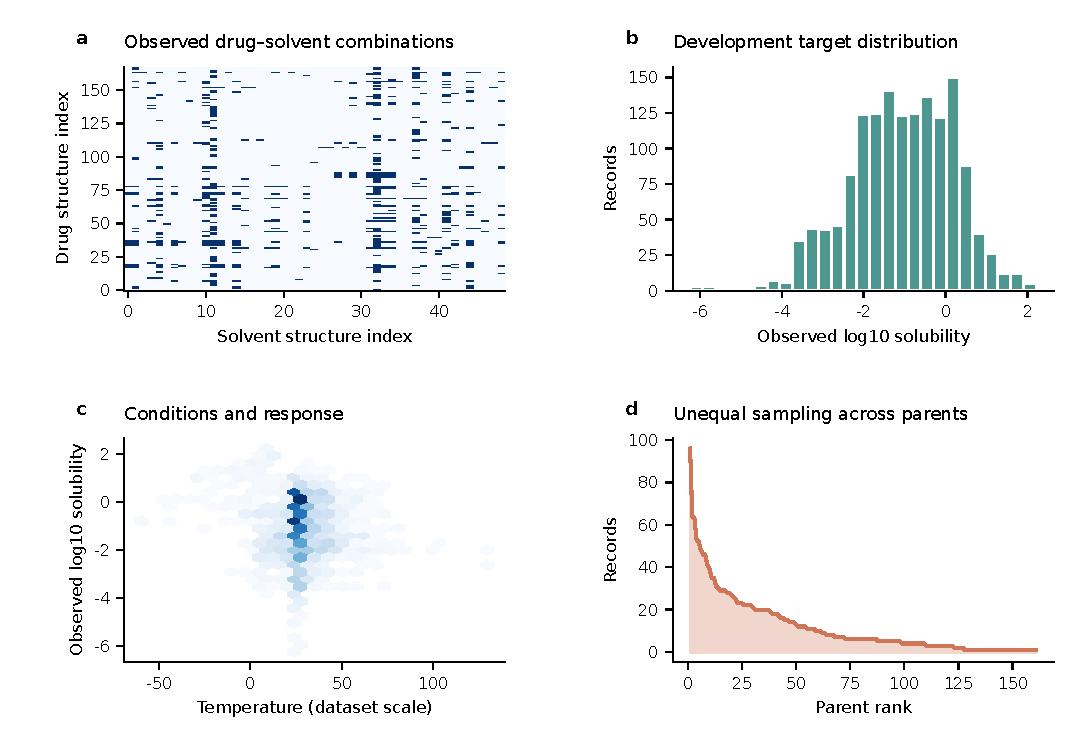
\includegraphics[width=\linewidth]{revision_v2/v2_data.pdf}
  \caption{Coverage, condition distribution, and sampling frequency of the dataset. \textbf{a} observed coverage of the drug--solvent combination grid; \textbf{b} log-solubility distribution of the development set; \textbf{c} joint temperature--solubility density; \textbf{d} descending per-parent sample counts.}
  \label{fig:v2-data-overview}
\end{figure}

Of the $168 \times 49 = 8232$ theoretical drug--solvent combinations, only 646 are actually observed, a global sparsity of 92.15\% (Figure~\ref{fig:v2-data-overview}a). Among these 646 combinations, 222 contain repeated measurements at several temperatures and account for 77.73\% of the rows, forming the core base for temperature-dependence analysis. The per-parent sample counts follow a sharp long-tail distribution (Figure~\ref{fig:v2-data-overview}d): 74 rare parents hold only 1--5 records each (182 records in total), while the top 30 parents each exceed 20 observations and monopolise 1078 records, 56.6\% of the dataset. Without reweighting and parent-equal evaluation, any conventional learner would inevitably overfit the head parents.

\subsection{Experimental Setup and Parent-Weighted Evaluation}\label{sec:v2-experiments}

\subsubsection{Nested Parent Holdout Design}
To balance strict anti-leakage against data use, the 161 parents are split in two: a core development set of 128 parents (1507 records) for model building, nested cross-validation, hyperparameter tuning, feature ablation, and blend-weight learning; and a held-out historical benchmark of 33 fully independent parents (397 records) as an unseen test library.

Within the development set, we adopt a strict five-outer/three-inner nested grouped cross-validation (Nested GroupKFold by parent). The outer loop splits parents into five folds, holding one out for unbiased evaluation; inside each outer training set, parents are again split into three inner folds, and all standardisation, imputation, dimensionality reduction, hyperparameter search, and blend-weight selection happen inside the inner loop\cite{varma2006,cawley2010}, keeping the outer validation fold invisible throughout. The outer models are refit under three random seeds (2026, 17, 42) to gauge the variance from algorithmic randomness.

\subsubsection{Parent-Weighted Risk and Sample Reweighting}
To counter long-tailed sampling, we formalise a parent-weighted empirical risk. Let $\mathcal{G}$ be the validation parents and $I_g$ the indices of all samples belonging to parent $g \in \mathcal{G}$. The evaluation loss is
\begin{equation}\label{eq:v2-common-risk}
\mathcal{L}_{\mathcal{G}}(f) = \frac{1}{|\mathcal{G}|} \sum_{g \in \mathcal{G}} \left( \frac{1}{|I_g|} \sum_{i \in I_g} |y_i - f(x_i)| \right).
\end{equation}
This criterion averages the absolute error inside each parent and then gives every parent exactly equal weight ($1/|\mathcal{G}|$), so that the metric reflects average generalisation over novel parents rather than being swayed by the parents with the most records.

To align the tree-splitting objective with this criterion, training uses the adaptive sample weight
\begin{equation}
w_i(q) = \frac{n_{g_i, \mathcal{T}}^{-q}}{N_{\mathcal{T}}^{-1} \sum_{j \in \mathcal{T}} n_{g_j, \mathcal{T}}^{-q}}, \qquad q \in \{0, 1\},
\label{eq:v2-train-weight}
\end{equation}
where $\mathcal{T}$ is the current training fold, $n_{g, \mathcal{T}}$ the number of samples of parent $g$ in $\mathcal{T}$, and $N_{\mathcal{T}} = |\mathcal{T}|$. With $q=0$ this reduces to ordinary row weighting; with $q=1$ each parent contributes a constant $N_{\mathcal{T}}/G_{\mathcal{T}}$ to the total loss regardless of how many records it has.

\subsubsection{Evaluation Metrics and Paired Inference}
Four metrics summarise the results. The parent-weighted mean absolute error (where $A_g = \frac{1}{|I_g|}\sum_{i\in I_g}|e_i|$ is parent $g$'s mean absolute error):
\begin{equation}
\mathrm{MAE}_{\mathrm{parent}} = \frac{1}{G}\sum_{g=1}^G A_g,
\end{equation}
the row-wise mean absolute error:
\begin{equation}
\mathrm{MAE}_{\mathrm{row}} = \frac{1}{N}\sum_{i=1}^N |e_i|,
\end{equation}
the root-mean-square error:
\begin{equation}
\mathrm{RMSE} = \sqrt{\frac{1}{N}\sum_{i=1}^N e_i^2},
\end{equation}
and the coefficient of determination:
\begin{equation}
R^2 = 1 - \frac{\sum_{i=1}^N e_i^2}{\sum_{i=1}^N (y_i - \bar y)^2}.
\end{equation}

Model comparisons use a non-parametric parent-paired bootstrap. Over 10,000 resamples of the 128 outer parents, we compute the paired difference $\Delta = \frac{1}{G}\sum_{g=1}^G (A_{g, A} - A_{g, B})$ and take the 2.5\% and 97.5\% quantiles as a 95\% confidence interval, which certifies the statistical significance of any improvement.

\subsection{Overall Architecture}

On a shared data structure and evaluation basis, this work builds and contrasts two complementary routes: SOLAR-H extracts the physical temperature slope by within-combination de-meaning, while ExtraTrees--TabPFN pursues high-dimensional explicit feature engineering and tabular-model blending (overview in Figure~\ref{fig:v2-method-workflows}).

\begin{figure}[htbp]
\centering
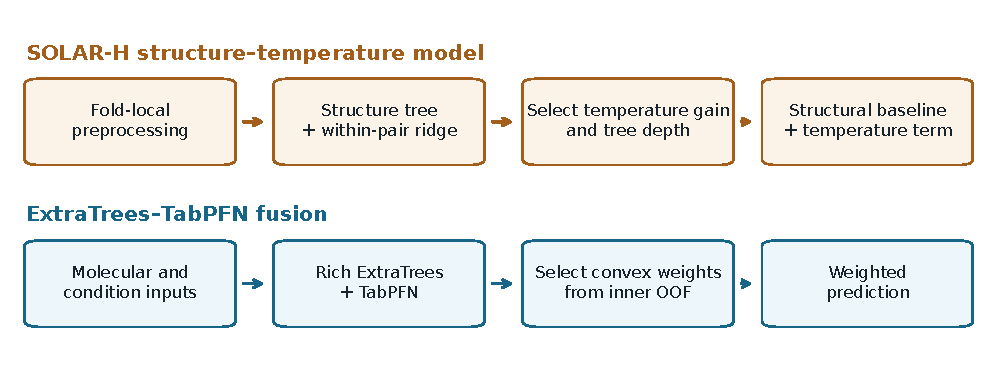
\includegraphics[width=\linewidth]{method_workflows.pdf}
\caption{Overview of the two technical routes for conditional solubility prediction.}
\label{fig:v2-method-workflows}
\end{figure}

\section{The SOLAR-H Structure--Temperature Decomposition Model}\label{sec:solar-method}

\subsection{Design Motivation}

In physical chemistry, dissolution is governed by solid--liquid equilibrium thermodynamics. The classical van 't Hoff equation ties the molar solubility to temperature through the apparent enthalpy of dissolution:
\begin{equation}
\frac{\partial \ln S}{\partial (1/T)} = -\frac{\Delta H_{\mathrm{sol}}}{R}.
\end{equation}
Over a limited operating window, a first-order Taylor approximation implies that the log-solubility depends quasi-linearly on the temperature displacement from a reference point. More importantly, $\Delta H_{\mathrm{sol}}$ is set by the difference between the solute--solvent solvation forces and the solute lattice energy, and is therefore strongly structure-specific.

A conventional regressor that feeds temperature in as one column among many molecular features confuses temperature variation with the absolute solubility differences between parents---temperature occupies only one dimension and each combination is measured over a different range---so the learned temperature response drifts badly on unseen parents. SOLAR-H (Structured Orthogonal Linear \& Additive Regression -- Hybrid) decouples the two: the local temperature slope is estimated orthogonally from within-combination temperature variation, and a tree ensemble then fits the structural baseline on a temperature-corrected target.

\subsection{Structure--Temperature Decomposition}

For the $i$-th record's combination $c_i$, we extract 11 base physicochemical descriptors for the drug and the solvent (molecular weight, MolLogP, TPSA, hydrogen-bond donors/acceptors, aromatic-ring count, and so on), standardise them per training fold, and form a 44-dimensional structural vector $z_c$ that combines the raw values, the Hadamard products, and the absolute differences. Adding a bias term gives the augmented vector $u_c = [1; z_c] \in \mathbb{R}^{45}$.

The temperature is robustly standardised with the training median $T_0$ and interquartile range $s_T$:
\begin{equation}
\tau_i = \frac{T_i - T_0}{s_T}.
\end{equation}
SOLAR-H expresses the predicted log-solubility as an additive combination of a structural baseline and a temperature response:
\begin{equation}\label{eq:v2-solar}
\widehat y_i = b(z_c) + \gamma \cdot \tau_i \cdot \left( u_c^\top \beta \right),
\end{equation}
where $b(z_c)$ is the nonlinear structural baseline at the reference temperature ($\tau_i = 0$, i.e.\ $T_i = T_0$) fitted by ExtraTrees, $u_c^\top \beta$ the local temperature slope of combination $c$, $\beta \in \mathbb{R}^{45}$ the structural modulation coefficients, and $\gamma \in [0, 1]$ the global temperature-gain shrinkage.

\subsection{Within-Group De-meaning Estimation}

The hard part is that the unknown baseline $b(z_c)$ is highly nonlinear; optimising it jointly would let the enormous absolute solubility differences between molecules swamp $\beta$.

SOLAR-H therefore borrows the fixed-effects device from panel-data econometrics. For each training combination $c$ with at least two distinct temperatures, define the within-group means $\bar y_c = \frac{1}{|c|}\sum_{i \in c} y_i$ and $\bar\tau_c = \frac{1}{|c|}\sum_{i \in c} \tau_i$, and subtract them inside each combination:
\begin{equation}
(y_i - \bar y_c) = \left[ b(z_c) - b(z_c) \right] + \gamma (u_c^\top \beta) (\tau_i - \bar\tau_c) + (\varepsilon_i - \bar\varepsilon_c).
\end{equation}
The unknown nonlinear baseline $b(z_c)$ cancels exactly. With the demeaned label $\Delta y_i = y_i - \bar y_c$ and the demeaned feature vector $A_i = (\tau_i - \bar\tau_c) u_c^\top \in \mathbb{R}^{45}$, and under the base gain $\gamma = 1$, estimating $\beta$ reduces to a parent-weighted ridge regression with $\ell_2$ regularisation:
\begin{equation}
\widehat\beta = \arg\min_\beta \sum_{i: |\Delta\tau_i| > 0} w_i(q=1) (\Delta y_i - A_i \beta)^2 + \lambda \|\beta\|_2^2.
\end{equation}
Setting the gradient to zero gives the closed form
\begin{equation}
\widehat\beta = (A^\top W A + \lambda I)^{-1} A^\top W \Delta y,
\end{equation}
where $W$ is the diagonal matrix of parent-equal weights $w_i(q=1)$ (Eq.~\eqref{eq:v2-train-weight}) and $\lambda$ the ridge penalty (fixed at 1000 for numerical stability of the inverse). Because the estimator strips away the absolute solubility differences between parents and uses only the temperature-driven within-system variation, it recovers the physical temperature effect without bias.

\subsection{Structural Baseline and Joint Fitting}

Once $\widehat\beta$ is available, the temperature contribution of every training sample is $\widehat\delta_i(\gamma) = \gamma \tau_i u_c^\top \widehat\beta$, and the corrected structural-baseline target is
\begin{equation}
\widetilde y_i(\gamma) = y_i - \widehat\delta_i(\gamma).
\end{equation}
A parent-weighted ExtraTrees ensemble (200 trees, minimum leaf size 1) is then trained on $\widetilde y_i$ to give $\widehat b(z_c)$. Inside the three-fold nested validation, we grid-search the tree-depth ceiling (8, 16, unbounded) jointly with the temperature gain $\gamma \in \{0, 0.1, 0.3, 1.0\}$, selecting by parent-weighted MAE; the chosen configuration is refit on the outer training set.

\subsection{Ablation and Adaptive Gain}

To isolate the contribution of each SOLAR-H module to cross-parent generalisation, we run a systematic ablation under the outer five-fold cross-validation, holding the parent split, test set, and seeds fixed while toggling parent weighting ($q=0$), the explicit interaction features, the temperature term entirely ($\gamma=0$), and a forced full gain ($\gamma=1$). The results and the paired-bootstrap 95\% intervals appear in Figure~\ref{fig:v2-solar-ablation}.

\begin{figure}[htbp]
\centering
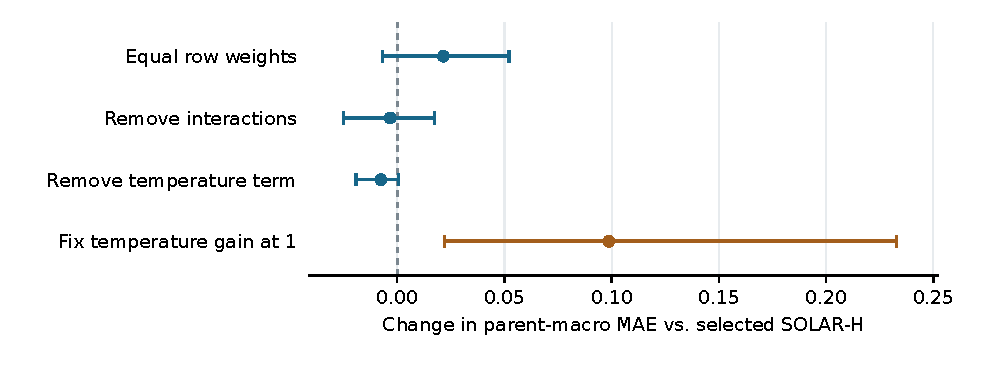
\includegraphics[width=\linewidth]{solar_ablation.pdf}
\caption{Ablation of the core SOLAR-H mechanisms. Points show each configuration's change in parent-weighted MAE relative to the adaptive baseline (positive means larger error); bars are 95\% intervals from 10,000 parent-paired bootstrap resamples.}
\label{fig:v2-solar-ablation}
\end{figure}

The ablation exposes the generalisation mechanism. Turning off parent weighting pushes the MAE on unseen parents to 0.7380 (up 0.0216), confirming that reweighting is what tames the frequent parents and secures the baseline for rare ones. The gain term matters even more: forcing the full gain ($\gamma = 1.0$) sends the MAE to 0.8150 (a deterioration of 0.0987), because the narrow temperature windows of small-sample combinations are easily perturbed by measurement noise; the adaptive shrinkage chosen inside the nested validation ($\gamma \in \{0, 0.1\}$) suppresses this over-extrapolation and keeps the learned temperature response stable.

\subsection{Summary}

This chapter built SOLAR-H, a decomposition that is both thermodynamically interpretable and statistically rigorous: within-group fixed effects remove the structural-baseline confounding, a weighted ridge regression yields a closed-form slope, and the nested validation pins down the adaptive gain. The ablations not only justify each component but also point to a methodological rule---extrapolating a physical slope to unseen scaffolds requires adaptive damping.

\section{The ExtraTrees--TabPFN Model with Feature Augmentation and Heterogeneous Blending}\label{sec:v2-methods}

\subsection{Design Motivation}

To lift the accuracy of conditional-solubility prediction on unseen parents, this chapter walks through a progressive refinement spanning feature representation, learning criterion, and heterogeneous ensembling. Three objectives drive it: build high-dimensional explicit solute--solvent interaction features along the like-dissolves-like principle to break the ceiling of naive concatenation; inject the parent-equal prior into the tree-splitting criterion to correct long-tailed sampling bias; and bring in the pretrained tabular foundation model TabPFN v2, whose attention-based metric mechanism complements the orthogonal splits of decision trees through an out-of-fold non-negative convex blend.

\subsection{Base ExtraTrees Model}

Starting from the input defined in Section~\ref{sec:v2-common-problem}, the base model takes 11 physicochemical properties for the drug and 11 for the solvent, plus the measurement temperature, forming a 23-dimensional vector $[D_i; S_i; T_i]$.

For the learner we adopt Extremely Randomized Trees (ExtraTrees\cite{extratrees2006}). Unlike a standard random forest, ExtraTrees draws not only a random feature subset at each node but also fully random split thresholds within the feature's range, then keeps the split with the largest weighted variance reduction. This threshold randomisation pays off in cheminformatics: it smooths the regression staircase instead of fitting hard step boundaries, and it decorrelates the base learners, giving better variance control than a random forest under the collinearity of high-dimensional molecular descriptors. The base model uses 200 trees with row-equal weighting and serves as the reference for every later modification.

\subsection{Descriptors and Explicit Interaction Features}

To supply richer chemical information, the feature space grows from 11 base properties to the full 217 descriptors extracted by RDKit, spanning topological indices (BalabanJ, Chi), electronic structure (PEOE, partial charges), polar surface (LabuteASA, TPSA), and functional-group counts. Let the standardised drug and solvent descriptors be $D_i \in \mathbb{R}^{217}$ and $S_i \in \mathbb{R}^{217}$.

The next step addresses a fundamental shortcoming of the naive concatenation $[D_i; S_i; T_i]$ (435 dimensions): it fails to capture intermolecular interactions. In solution thermodynamics, dissolution reflects the competition among solute--solute, solvent--solvent, and solute--solvent interactions. Along the like-dissolves-like principle, the absolute-difference vector $|D_i - S_i|$ measures the mismatch between solute and solvent on matching physicochemical dimensions (polarity mismatch $|\mathrm{TPSA}_D - \mathrm{TPSA}_S|$, lipophilicity mismatch $|\mathrm{MolLogP}_D - \mathrm{MolLogP}_S|$; smaller means more compatible), while the Hadamard product $D_i \odot S_i$ measures the conjugated enhancement on specific thermodynamic properties (hydrogen-bond donor/acceptor interplay).

Leaving these interactions for the tree to discover implicitly would cost two or more orthogonal splits just to approximate a simple difference. We therefore build an 869-dimensional explicit interaction space:
\begin{equation}
x_i^{\mathrm{int}} = \left[ D_i;\; S_i;\; T_i;\; D_i \odot S_i;\; |D_i - S_i| \right] \in \mathbb{R}^{869}.
\end{equation}
Adding the standardised parent-scaffold descriptors yields a candidate 1086-dimensional representation. In the feature pipeline, median imputation and zero-variance filtering for the few malformed molecules are fitted strictly inside each inner training fold, leaving 665 dense, informative features and ruling out leakage.

\subsection{Parent-Weighted Optimisation}

To make ExtraTrees robust to long-tailed sampling, the parent weights $w_i(q)$ of Eq.~\eqref{eq:v2-train-weight} are plugged directly into the node-splitting algorithm. At a node $L$ the weighted sum of squared deviations is
\begin{equation}
J_L(v) = \sum_{i \in L} w_i(q) (y_i - v)^2.
\end{equation}
Setting $\frac{\partial J_L}{\partial v} = 0$ shows that the optimal leaf prediction is the weighted mean
\begin{equation}
\widehat v_L = \frac{\sum_{i \in L} w_i(q) y_i}{\sum_{i \in L} w_i(q)}.
\end{equation}
When a candidate split divides a parent $P$ into a left child $L$ and a right child $R$, its weighted impurity drop is
\begin{equation}
\Delta J(s) = J_P(\widehat v_P) - \left[ \frac{\sum_{i \in L} w_i}{\sum_{i \in P} w_i} J_L(\widehat v_L) + \frac{\sum_{i \in R} w_i}{\sum_{i \in P} w_i} J_R(\widehat v_R) \right].
\end{equation}
With $q=1$, every parent contributes the same total effective sample mass during tree growth: dense records inside a frequent parent can only refine local micro-splits and cannot dominate the rare parents at the macro level. The refined ExtraTrees uses 300 trees, a feature-sampling ratio of 0.7, a minimum leaf size of 2, and unrestricted depth.

\subsection{TabPFN Foundation Model}

As a heterogeneous complement to the tree ensemble, we incorporate the recent tabular foundation model TabPFN v2\cite{tabpfn2025}.

Pretrained via an autoregressive Transformer on millions of synthetic causal-topology prior datasets, TabPFN keeps its network parameters fixed at inference and takes the whole labelled training set as context:
\begin{equation}
\mathcal{C}_{\mathcal{T}} = \left\{ (x_i, y_i) \mid i \in \mathcal{T} \right\}.
\end{equation}
For a query condition $x^*$, it attends over all context samples and returns the posterior mean of the Bayesian predictive distribution:
\begin{equation}
f_{\mathrm{PFN}}(x^*) = \mathbb{E}_{\theta}\left[ Y \mid x^*, \mathcal{C}_{\mathcal{T}} \right].
\end{equation}
TabPFN's smooth attention-distance inductive bias captures gradual transitions in continuous space, whereas ExtraTrees builds staircase boundaries on high-dimensional sparse features through orthogonal splits. The two are highly independent in mechanism and in error distribution.

\subsection{Out-of-Fold Non-negative Convex Blending}

To blend ExtraTrees and TabPFN optimally without the second-order overfitting that comes from tuning the weight on the training set, we design an out-of-fold (OOF) non-negative convex combination. Inside the 3-fold split of the outer training set, let $t_i$ and $p_i$ be the ExtraTrees and TabPFN predictions of record $i$ on its held-out inner fold. The blended prediction is
\begin{equation}
\widehat y_i(\alpha) = (1 - \alpha) t_i + \alpha p_i = t_i + \alpha (p_i - t_i),
\end{equation}
where $(p_i - t_i)$ is TabPFN's correction to the tree baseline and $\alpha \in [0, 1]$ the blend weight. Substituting this into the parent-weighted risk (Eq.~\eqref{eq:v2-common-risk}) gives a constrained minimisation:
\begin{equation}
\widehat\alpha = \arg\min_{\alpha \in \{0, 0.25, 0.5, 0.75, 1.0\}} \frac{1}{|\mathcal{G}_{\mathrm{in}}|} \sum_{g \in \mathcal{G}_{\mathrm{in}}} \left( \frac{1}{|I_g|} \sum_{i \in I_g} \left| y_i - \left[ (1 - \alpha) t_i + \alpha p_i \right] \right| \right).
\label{eq:v2-blend-selection}
\end{equation}
A grid search picks the optimal step $\widehat\alpha$; $\widehat\alpha = 0$ collapses to the pure tree and $\widehat\alpha = 1$ to pure TabPFN. After the weight is chosen per outer fold, both learners are refit on the full outer data, and the final ensemble predicts
\begin{equation}
\widehat y(x) = (1 - \widehat\alpha) f_{\mathrm{ET}}(x) + \widehat\alpha f_{\mathrm{PFN}}(x).
\label{eq:v2-prediction-blend}
\end{equation}

\subsection{Ablation}

Holding the inner three-fold grouping and seed 2026 fixed on the development set, Table~\ref{tab:v2_tree_pilot} reports the progressive ablation of the core ExtraTrees designs.

\begin{table}[htbp]
\centering
\small
\caption{Ablation of the core ExtraTrees designs (values are parent-weighted MAE).}
\label{tab:v2_tree_pilot}
\begin{tabular}{lrr}
\toprule
Input representation & Row-equal ($q=0$) & Parent-equal ($q=1$) \\
\midrule
435-dim descriptor concatenation & 0.7112 & 0.6853 \\
869-dim explicit interactions (concat, product, absolute difference) & \textbf{0.6985} & \textbf{0.6760} \\
\bottomrule
\end{tabular}
\end{table}

The ablation confirms the incremental gain of each module. Relative to the plain concatenation, adding the absolute differences and products lowers the parent-weighted MAE by about 0.01, evidence that explicit interactions spare the tree from searching for them. Switching to parent-equal training brings a further reduction of over 0.022, confirming that the objective correction is necessary. On the TabPFN side, compressing the context to 8 or 16 records per parent worsens the MAE to above 0.74, while the full context lets the model exploit its large-sample background. The final out-of-fold two-branch blend again beats either single model, validating the complementarity of the heterogeneous ensemble.

Two practical issues were handled along the way. Non-finite descriptor values caused by dense heteroatoms are addressed with median imputation and dynamic variance filtering, fitted strictly inside each fold; the storage cost of TabPFN's large context is mitigated with dynamic memory release and GPU acceleration, bringing single inference below one second.

\subsection{Summary}

This chapter derived the ExtraTrees--TabPFN architecture and its progressive refinements. The experiments confirm that the 869-dimensional explicit physicochemical interactions, the parent-equal tree splitting, and the out-of-fold convex blending together build a heterogeneous ensemble that is both accurate and mechanistically complementary.

\section{Model Comparison and Generalisation Analysis}

\subsection{Experimental Setup and Baselines}

To assess generalisation and design effectiveness fairly, every model is evaluated under the outer five-fold parent split established in Section~\ref{sec:v2-experiments}. All candidates share exactly the same training and held-out parent partitions, are refit under three independent seeds (2026, 17, 42), and report the average of the three seeds.

To form a multi-level, multi-paradigm benchmark, we assemble the comparison matrix in Table~\ref{tab:v2-experiment-matrix}.

\begin{table}[htbp]
  \centering\small
  \caption{Comparison matrix of models and their hyperparameter search spaces.}
  \label{tab:v2-experiment-matrix}
  \begin{tabularx}{\linewidth}{@{}lllX@{}}
    \toprule
    Category & Model & Input dimension & Tuning space and mechanism \\
    \midrule
    \multirow{2}{*}{Conventional single models}
    & Base ExtraTrees baseline & 23 (base descriptors + temperature) & 12 tree-hyperparameter combinations (depth 8--unbounded, leaf 1--4, feature ratio 0.5--1.0). \\
    & Feature-rich ExtraTrees & 869 (explicit interactions) & 3 representations $\times$ 2 weightings ($q \in \{0, 1\}$), 6 configurations. \\
    \midrule
    Physical decomposition & SOLAR-H & 45 (augmented) & 4 temperature gains ($\gamma \in \{0, 0.1, 0.3, 1.0\}$) $\times$ 3 tree depths, 12 configurations. \\
    \midrule
    \multirow{3}{*}{Recent single models}
    & TabPFN v2 & 23 / 435 & 2 input dimensions $\times$ 2 internal ensemble sizes (2, 4), 4 configurations. \\
    & CatBoost & 869 (interactions) & 6 depth/learning-rate combinations (symmetric depth 4--8, L2 1--10)\cite{catboost2018}. \\
    & TabM deep tabular network & 869 (interactions) & parameter-efficient multi-head tabular architecture (2 hidden-layer settings)\cite{tabm2025}. \\
    & Multi-view kernel ridge & multiple topological and physicochemical kernels & graph fingerprints plus physicochemical kernels, 10 regularisation values. \\
    \midrule
    \multirow{3}{*}{Ensembles}
    & \textbf{ExtraTrees--TabPFN (ours)} & heterogeneous two-branch & adaptive non-negative convex weight $\alpha \in [0, 1]$ on inner OOF predictions (step 0.25). \\
    & Three-branch blend & ET + CatBoost + TabPFN & Dirichlet grid search over the three non-negative convex weights. \\
    & Five-branch blend & all candidate learners & full search over two tree ensembles, the deep tabular network, kernels, and TabPFN. \\
    \bottomrule
  \end{tabularx}
\end{table}

All hyperparameter tuning and weight selection are sealed inside the inner three-fold loop, so the out-of-fold predictions on the 128 outer test parents are genuinely blind. This protocol keeps the comparison conclusions highly reliable.

\subsection{Overall Performance}\label{sec:prediction_results}

Under the strict outer cross-validation over 128 unseen parents and 1507 development records, Table~\ref{tab:v2_main_metrics} summarises the baselines and the proposed models.

\begin{table}[htbp]
\centering
\small
\caption{Overall performance under the parent-grouped outer nested validation on the development set (the first three columns are log-solubility errors, lower is better; higher $R^2$ is better).}
\label{tab:v2_main_metrics}
\begin{tabular}{lrrrr}
\toprule
Model & Parent-weighted MAE & Row-wise MAE & RMSE & $R^2$ \\
\midrule
Ridge regression & 0.8746 & 0.9155 & 1.2087 & 0.1094 \\
TabM deep tabular network & 0.7694 & 0.7679 & 1.0104 & 0.3777 \\
Base ExtraTrees baseline & 0.7469 & 0.7491 & 0.9730 & 0.4229 \\
Multi-view kernel ridge & 0.7277 & 0.7388 & 0.9501 & 0.4497 \\
RBF support-vector regression & 0.7226 & 0.6600 & 0.9125 & 0.4924 \\
SOLAR-H structure--temperature decomposition & 0.7164 & 0.7520 & 1.0016 & 0.3884 \\
CatBoost gradient boosting & 0.6931 & 0.7168 & 0.9462 & 0.4542 \\
Feature-rich ExtraTrees & 0.6831 & 0.6720 & 0.8981 & 0.5083 \\
TabPFN v2 single branch & 0.6827 & 0.6698 & 0.9117 & 0.4933 \\
Random forest & 0.6815 & 0.7057 & 0.9254 & 0.4780 \\
\midrule
TabPFN + two-tree (ET+CatBoost) three-blend & 0.6729 & 0.6631 & 0.8882 & 0.5191 \\
Five-branch full blend & 0.6767 & 0.6568 & 0.8899 & 0.5172 \\
\textbf{ExtraTrees--TabPFN blend (recommended)} & \textbf{0.6668} & \textbf{0.6510} & \textbf{0.8842} & \textbf{0.5234} \\
\bottomrule
\end{tabular}
\end{table}

Across all metrics, the proposed ExtraTrees--TabPFN blend leads the field: its parent-weighted MAE (0.6668), row-wise MAE (0.6510), RMSE (0.8842), and $R^2$ (0.5234) all rank first. Against the base ExtraTrees baseline, the parent MAE drops by 8.54\% (paired 95\% interval $[-0.1219, -0.0082]$), a statistically solid improvement.

The jump from single models to the blend shows the complementarity dividend. ExtraTrees and TabPFN perform similarly alone on unseen parents (MAE 0.6831 versus 0.6827), yet their residual signs disagree 15.0\% of the time and their predictions correlate at only 0.909. The out-of-fold convex combination converts this orthogonality into variance suppression, pushing the parent MAE further down to 0.6668.

SOLAR-H reaches a parent MAE of 0.7164. It trails the blend but beats the base tree baseline clearly (paired difference $+0.0496$), and by cleanly decoupling the conditional solubility into an interpretable physical temperature response and a structural baseline, it supplies the theoretical reference that the later causal analysis relies on.

To render the multi-metric standing of each model at a glance, Figure~\ref{fig:model_radar} shows the same comparison as a normalised radar profile.

\begin{figure}[htbp]
\centering
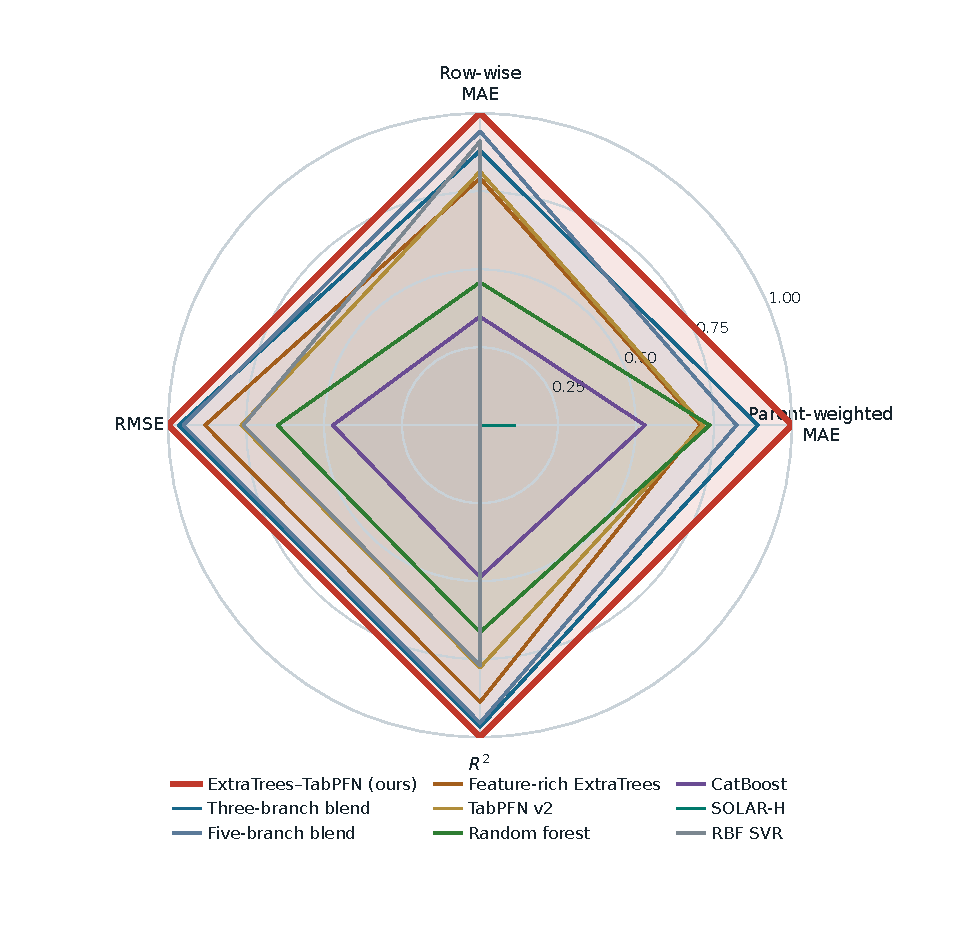
\includegraphics[width=0.78\linewidth]{model_radar.pdf}
\caption{Normalised radar comparison of the models across the four metrics (all axes are normalised to $[0,1]$ with a larger radius always better; the three error metrics are inverted).}
\label{fig:model_radar}
\end{figure}

\subsection{Ablation Analysis}

Figure~\ref{fig:v2_prediction_diagnostics}a shows the paired gains of the blend over its baselines together with the bootstrap intervals.

\begin{figure}[htbp]
\centering
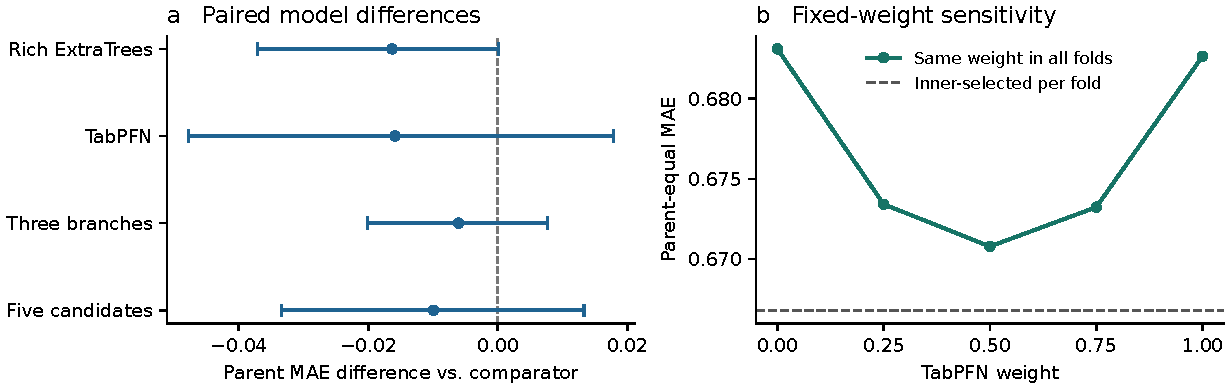
\includegraphics[width=\linewidth]{prediction_diagnostics.pdf}
\caption{Performance gains and weight sensitivity of the ExtraTrees--TabPFN blend. \textbf{a} paired differences in parent-weighted MAE against the baselines (negative means the blend is better; bars are 95\% bootstrap intervals). \textbf{b} parent MAE as a function of a fixed global weight $\alpha$ (the dashed line is the adaptive per-fold baseline).}
\label{fig:v2_prediction_diagnostics}
\end{figure}

Tracing the whole technical trajectory, three core refinements drive the gains: the leap from 23 base features to 869 explicit interaction features, which feeds polarity matching directly and narrows the error; the parent-equal sample weighting ($q=1$), which removes the head-parent bias and cuts the error by a further 0.023; and the context-attention TabPFN branch, which applies a local continuous correction and locks the parent MAE at the global optimum of 0.6668.

\subsection{Stratified Error Analysis}

At the parent level, the median per-parent MAE of SOLAR-H and the blend over the 128 unseen parents are 0.599 and 0.544. Across all 128 test parents, the blend beats SOLAR-H on 77 parents and beats the feature-rich ExtraTrees single model on 61.

To understand the behaviour across physicochemical environments, Table~\ref{tab:v2_target_band_errors} reports the two models' errors stratified by the measured log-solubility band.

\begin{table}[htbp]
\centering
\small
\setlength{\tabcolsep}{3.5pt}
\caption{Stratified errors of the two core models across measured-solubility bands (signed error is prediction minus measurement; positive means systematic overestimation, negative underestimation).}
\label{tab:v2_target_band_errors}
\begin{tabular}{lrrrrrr}
\toprule
& & & \multicolumn{2}{c}{SOLAR-H} & \multicolumn{2}{c}{ExtraTrees--TabPFN}\\
\cmidrule(lr){4-5}\cmidrule(lr){6-7}
Band & Records & Parents & Row-wise MAE & Signed error & Row-wise MAE & Signed error \\
\midrule
Extreme ($y \leqslant -4$) & 23 & 8 & 2.413 & $+2.396$ & 2.251 & $+2.250$ \\
Low ($-4 < y \leqslant -2$) & 321 & 56 & 0.997 & $+0.876$ & 0.874 & $+0.784$ \\
Moderate ($-2 < y \leqslant 0$) & 824 & 110 & \textbf{0.551} & $-0.184$ & \textbf{0.465} & $-0.120$ \\
High ($y > 0$) & 339 & 43 & 0.895 & $-0.873$ & 0.782 & $-0.772$ \\
\bottomrule
\end{tabular}
\end{table}

The stratified errors expose a chemically meaningful ``solubility cliff''.

In the moderate band ($-2 < y \le 0$), which holds 54.7\% of the samples, the blend performs exceptionally well---a row-wise MAE of just 0.465 and a signed bias of $-0.120$---delivering accurate continuous fits for routine pharmaceutical conditions.

In the extreme band ($y \le -4$, 23 records over 8 parents), both models' errors balloon (MAE above 2.2) and both systematically overestimate by more than $+2.2$ orders of magnitude. Take sucrose in chloroform at $25^\circ\text{C}$: the measured log-solubility is $-6.234$, but the model predicts $-2.536$ on average. The mechanism is thermodynamic: solubility depends not only on the liquid-phase solvation free energy (captured by 2D topological descriptors) but also, and more directly, on the lattice energy and solid-state packing of the pure crystal. Sucrose carries abundant hydroxyl groups that form a strong interlocking hydrogen-bond network in the solid, so desolvation and melting must overcome a large lattice-energy barrier, which is why it is so insoluble in chloroform. A pure 2D prediction, without an experimental melting point or three-dimensional unit-cell packing parameters, can only reason from liquid-phase polarity mismatch and therefore overestimates systematically. This is a practically important warning: for compounds predicted near the insoluble edge, solid-state polymorph and melting-point measurement should be scheduled first.

\subsection{Sensitivity and Randomness}

Across the outer five folds, the adaptively chosen TabPFN blend weights $\widehat\alpha$ are 0.25, 0.25, 0.0, 0.25, 0.50 (averaging about 0.25), and the ExtraTrees weighting exponent $q$ consistently prefers 1.

On weight robustness, Figure~\ref{fig:v2_prediction_diagnostics}b fixes the out-of-fold predictions and sweeps a constant global $\alpha$. Over $\alpha \in [0.25, 0.75]$ the parent-weighted MAE is 0.6734, 0.6708, 0.6732---a very flat basin that beats both single-branch endpoints (0.6831 at $\alpha=0$ and 0.6827 at $\alpha=1$). The blending gain is therefore tolerant of weight changes rather than depending on a brittle optimum.

On seed sensitivity, holding the same five-fold parent split and reporting seeds 17, 42, and 2026, the blend's parent-weighted MAEs are 0.6635, 0.6679, and 0.6690---a spread of only 0.0055. This low random variance confirms the stability of both the training strategy and the ensemble.

\subsection{Model Selection and Deployment}

Enlarging the candidate pool does not help. Adding CatBoost to form a three-branch ensemble gives a parent MAE of 0.6729; using all five candidate learners gives 0.6767. Both trail the two-branch ExtraTrees--TabPFN (0.6668).

Following Occam's razor, we therefore keep the two-branch blend as the final model. It holds the best generalisation and the lowest dispersion; relative to the three- or five-branch variants it avoids model bloat and storage overflow while simplifying the system, and under GPU acceleration it responds in under a second, which suits interactive real-time screening.

\section{Model Interpretability and the Role of Temperature}

\subsection{Analysis Objectives}

In drug discovery and process design, an accurate model without transparent decision logic will struggle to earn a medicinal chemist's trust, let alone guide molecular modification or process changes. This chapter addresses two mechanistic questions: the feature attribution of ExtraTrees--TabPFN and the local corrections made by TabPFN, and the physical causal link between temperature and solubility.

\subsection{Structural Contributions in SOLAR-H}

SOLAR-H is white-box by construction. From Eq.~\eqref{eq:v2-solar} the output is a linear superposition of two terms:
\begin{equation}
\widehat y_i = \underbrace{\widehat b(z_c)}_{\text{structural constant}} + \underbrace{\gamma \cdot \tau_i \cdot \left( u_c^\top \widehat\beta \right)}_{\text{structure-modulated temperature response}}.
\end{equation}
For any fixed combination $c$ the temperature derivative is constant, $\frac{\partial \widehat y}{\partial T} = \frac{\gamma u_c^\top \widehat\beta}{s_T}$. In the full development deployment, the nested validation selects the high-damping gain $\gamma = 0$, so the model degenerates to a structural-baseline prediction and avoids extrapolation drift from temperature noise on unseen parents. With a non-zero gain on the training folds, $\widehat\beta$ reveals how molecular-weight differences and polarity mismatch steer the endothermic slope.

\subsection{Feature Attribution}\label{sec:deployment-explanations}

For the nonlinear ExtraTrees--TabPFN deployed model, we combine game-theoretic Shapley values with local branch contributions in a two-pronged attribution.

\subsubsection{TreeSHAP Global Feature-Group Attribution}
For the ExtraTrees branch we use the tree-path-dependent TreeSHAP algorithm\cite{treeshap2020}, drawing 227 explanation samples that evenly cover the chemical space of the 128 development parents. TreeSHAP satisfies the local-accuracy axiom to floating-point precision (reconstruction bias below $1.3\times10^{-13}$), with a background expectation of $-1.1632$.

The 665 retained features fall into four groups: drug descriptors, solvent descriptors, temperature, and explicit intermolecular interactions. Each group's signed attribution is averaged equally over the 128 parents (Figure~\ref{fig:deployment-explanations}A).

\begin{figure}[htbp]
\centering
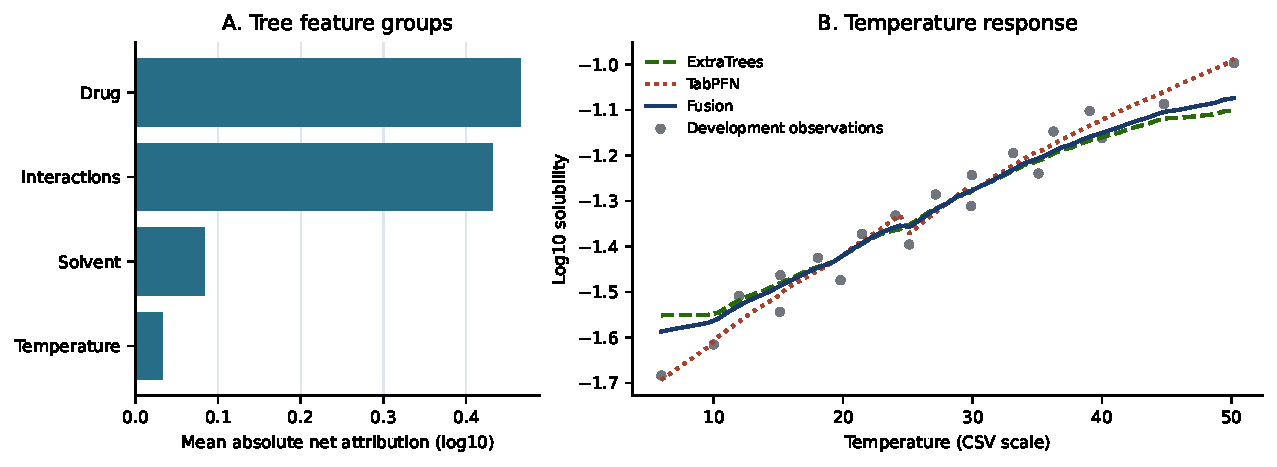
\includegraphics[width=\linewidth]{deployment_explanations.pdf}
\caption{Feature attribution and dynamic temperature response of the deployed model. \textbf{A} parent-equal absolute net attribution of the four feature groups; \textbf{B} predicted curve for the lovastatin--butyl acetate combination over its observed temperature window (markers are measurements, the solid line is the blend, dashed lines are the single branches).}
\label{fig:deployment-explanations}
\end{figure}

The attribution is chemically interpretable. Drug descriptors (mean absolute attribution 0.466) and explicit interaction features (0.432) contribute most to the predictions. This matches solution physicochemical principles: drug molecules are large and complex (molecular weights usually 200--800), and their lattice energy and solid-state cohesion are a barrier to dissolution; the explicit solute--solvent interactions (polarity matching and hydrogen bonding) then decide whether solvation can overcome that lattice energy. Solvent descriptors (0.084) and temperature (0.033) only fine-tune the prediction. Because the solvent library is small (49 common industrial solvents) and its structures are regular, the solvent's standalone contribution is concentrated and acts mostly as a conditional perturbation on the structural baseline.

\subsubsection{TabPFN's Local Branch Calibration}
To see how TabPFN cooperates with ExtraTrees, Table~\ref{tab:deployment-examples} picks two real cases where the TabPFN correction $\Delta_{\mathrm{PFN}} = 0.25 (f_{\mathrm{PFN}} - f_{\mathrm{ET}})$ takes extreme values in opposite directions.

\begin{table}[htbp]
\centering\small
\setlength{\tabcolsep}{4pt}
\caption{Two representative cases of TabPFN's bidirectional calibration of the ExtraTrees branch (both in acetone).}
\label{tab:deployment-examples}
\begin{tabular}{lrrrrrr}
\toprule
Drug (row) & Temperature ($^\circ\text{C}$) & Measured & ExtraTrees & TabPFN & Blend & Correction $\Delta_{\mathrm{PFN}}$ \\
\midrule
Erythritol (row 23) & 13.2 & $-2.692$ & $-2.495$ & $-2.716$ & $-2.551$ & $-0.055$ (down) \\
4-hydroxyphenylglycine Dane salt (row 3) & 70.2 & $-1.843$ & $-1.927$ & $-1.847$ & $-1.907$ & $+0.020$ (up) \\
\bottomrule
\end{tabular}
\end{table}

The two cases illustrate the ensemble's adaptive calibration. For erythritol, ExtraTrees is pulled toward the statistical mean of polyols at room temperature and predicts $-2.495$, a clear overestimate of the measured $-2.692$; TabPFN, attending over continuous space, recognises the insolubility of a highly polar small molecule in a low-polarity solvent and predicts $-2.716$, driving the blend down to $-2.551$ and cutting the error sharply. For the Dane salt, ExtraTrees is conservative ($-1.927$), while TabPFN picks up the thermodynamic solubilisation at $70.2^\circ\text{C}$ and predicts $-1.847$, nudging the blend up to $-1.907$, close to the measured $-1.843$. TabPFN thus applies corrections in opposite directions across different chemical spaces, drawing on its rich prior-manifold representation.

\subsection{Dynamic Temperature Response}

To check physical plausibility under continuous temperature change, we fix the lovastatin--butyl acetate system (20 dense temperature points in the development set, spanning $[5.95^\circ\text{C}, 50.2^\circ\text{C}]$) and scan the temperature densely (Figure~\ref{fig:deployment-explanations}B).

The temperature scan shows different behaviours: ExtraTrees produces a staircase of piecewise segments, as expected from an axis-split tree, while the blend traces a smooth, monotone upward curve whose log-solubility rises from $-1.587$ at $5.95^\circ\text{C}$ to $-1.074$ at $50.2^\circ\text{C}$. The curve passes through the middle of the observed scatter and matches the endothermic-dissolution behaviour of most solid solutes.

\subsection{Measured Temperature Association and Causal Identification}\label{sec:temperature-association}

\subsubsection{Causal Graph for the Temperature Effect}

In uncontrolled observational data, equating a statistical association with a physical temperature effect is risky. We therefore frame the analysis with a structural causal model (SCM)\cite{pearl2009}. Let $D$ and $S$ denote the drug and solvent structures, $T$ the temperature, $Y$ the log-solubility, and $U$ the unrecorded environmental and experimental confounders (measurement protocol, solid-state polymorph transitions, equilibration time, and so on).

The causal directed acyclic graph (DAG) is shown in Figure~\ref{fig:causal-dag}.
\begin{figure}[htbp]
\centering
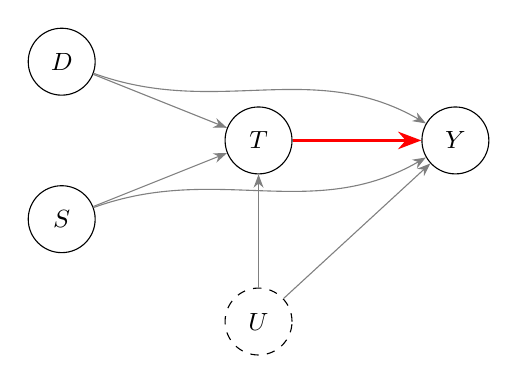
\begin{tikzpicture}[
  >=Stealth,
  obs/.style={draw, circle, minimum size=0.85cm, inner sep=0pt, font=\small},
  latent/.style={draw, circle, dashed, minimum size=0.85cm, inner sep=0pt, font=\small},
  causal/.style={->, red, very thick},
  arrow/.style={->, gray}
]
\node[obs] (D) at (0,2.0) {$D$};
\node[obs] (S) at (0,0.0) {$S$};
\node[obs] (T) at (2.5,1.0) {$T$};
\node[obs] (Y) at (5.0,1.0) {$Y$};
\node[latent] (U) at (2.5,-1.3) {$U$};
\draw[arrow] (D) -- (T);
\draw[arrow] (S) -- (T);
\draw[arrow] (D) to[out=-20, in=150] (Y);
\draw[arrow] (S) to[out=20, in=-150] (Y);
\draw[arrow] (U) -- (T);
\draw[arrow] (U) -- (Y);
\draw[causal] (T) -- (Y);
\end{tikzpicture}
\caption{Causal DAG for the temperature effect. Solid circles are observed variables, the dashed circle is the unmeasured confounder; the red arrow $T \to Y$ is the target causal path and the grey arrows are backdoor paths.}
\label{fig:causal-dag}
\end{figure}
In this graph the path $T \to Y$ is the causal response of interest, the change in log-solubility when the temperature changes. Two serious backdoor paths exist: the drug and solvent structures correlate with the temperature window chosen, giving the structural backdoor $T \leftarrow (D, S) \to Y$; and experiments at different temperatures may differ in their instrument protocols, giving the environmental backdoor $T \leftarrow U \to Y$.

\subsubsection{Resolving Simpson's Paradox}

To block the structural backdoor $T \leftarrow (D, S) \to Y$, we keep all complete drug--solvent combinations with at least two distinct temperatures: 157 combinations, 73 parents, and 1118 records (median temperature span $27.1^\circ\text{C}$).

On this set, contrasting two regressions exposes the distortion. The pooled ordinary least squares (OLS) yields $\widehat\beta_{\mathrm{pooled}} = -0.00746$ (Figure~\ref{fig:v2-temperature-associations}), a negative correlation that contradicts endothermic dissolution and betrays a Simpson's paradox. The sign flip stems from the correlation between temperature and insolubility in the sample: poorly soluble systems are measured more often at higher temperatures, which manufactures a spurious negative correlation at the pooled level.

Within-combination fixed-effects regression, by contrast, fits
\begin{equation}
Y_{ic} = \alpha_c + \beta_{\mathrm{within}} T_{ic} + \varepsilon_{ic}, \qquad \widehat\beta_{\mathrm{within}} = \frac{\sum_c\sum_i (T_{ic} - \bar T_c)(Y_{ic} - \bar Y_c)}{\sum_c\sum_i (T_{ic} - \bar T_c)^2}.
\end{equation}
De-meaning within each combination removes the structural intercept $\alpha_c$ entirely, blocking all temperature-invariant drug and solvent confounding.

\subsubsection{Within-Group Temperature Slope and Uncertainty}

The estimates appear in Figure~\ref{fig:v2-temperature-associations}. On exactly the same 1118 records, the within-combination fixed-effects slope is
\begin{equation}
\widehat\beta_{\mathrm{within}} = +0.01538.
\end{equation}
That is, each $1^\circ\text{C}$ increase raises the mean log-solubility by 0.01538, a net molar-solubility gain of about 3.6\%.

\begin{figure}[htbp]
\centering
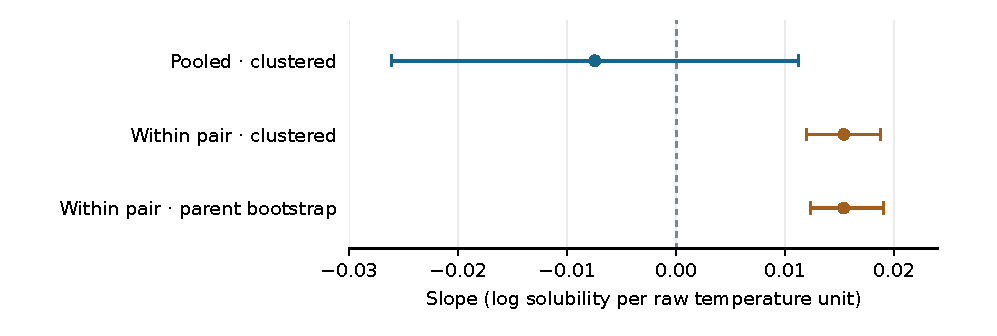
\includegraphics[width=\linewidth]{temperature_associations.pdf}
\caption{Statistical association and causal identification between temperature and measured log-solubility. The first row is the pooled OLS regression; the second and third rows are the within-combination fixed-effects slope and its confidence intervals.}
\label{fig:v2-temperature-associations}
\end{figure}

Three uncertainty analyses back the effect. With parent-clustered robust errors, the 95\% interval is strictly positive, $[0.0121, 0.0186]$; a parent-clustered bootstrap with 2000 resamples gives the percentile interval $[0.01236, 0.01902]$; and a leave-one-parent-out jackknife over the 73 parents keeps the slope within $[0.01424, 0.01599]$. All are positive, so the effect is robust across parents.

\subsubsection{Sensitivity to Unmeasured Confounding}

Fixed effects remove all structural invariants, but a temperature-varying unmeasured confounder $U$ (a polymorph transition or a different measurement time at different temperatures) could in principle still bias the estimate. We therefore apply the Cinelli--Hazlett sensitivity framework\cite{sensitivity2020}. Let $r_T^2$ be the partial $R^2$ of $U$ on $T$ after controlling for the combination effects, and $r_Y^2$ the partial $R^2$ of $U$ on $Y$. Using the omitted-variable-bias identity, we compute the minimal confounding strength needed to drive the adjusted temperature slope to zero (the robustness value). Under the worst-case same-direction bias, the requirement is
\begin{equation}
r_T^2 = r_Y^2 \approx 0.54.
\end{equation}
An unmeasured confounder would have to explain at least 54\% of the residual variance of both temperature and solubility to overturn the positive effect. That degree of co-variation is unlikely for instrument and operational variation in these measurements.

\subsection{Summary}

Taken together, these analyses establish a clear interpretive and causal picture. The ExtraTrees--TabPFN decisions depend mainly on the drug's intrinsic structure and on solute--solvent polarity and hydrogen-bond complementarity, in line with the molecular physicochemical mechanism of dissolution. Within-combination de-meaning resolves the Simpson's paradox in the observational data and pins down a trustworthy positive temperature slope ($+0.01538$), which informs process temperature optimisation. For extrapolation to entirely new parents, the temperature prediction remains a conditional statistical response; in a real crystallisation campaign, the critical points should be checked experimentally under standard operating procedures.

\section{System Design and Implementation}\label{sec:v2-application}

\subsection{System Architecture}

To put the proposed algorithms to practical use in drug discovery and crystallisation process design, we built a full-stack, high-availability, low-latency interactive system for conditional-solubility prediction and decision support, following modern software-engineering practice.

The system uses a cohesive, loosely coupled layered architecture (the end-to-end pipeline is shown in Figure~\ref{fig:v2-app-flow}). The presentation layer offers molecule lookup, single-point prediction, side-by-side model comparison, temperature scanning, and batch CSV. The service layer, built on FastAPI, handles contract validation and asynchronous concurrency. The feature engine assembles descriptors and explicit interaction vectors on the fly with RDKit. The inference engine keeps the models resident on CPU and GPU for millisecond-level responses.

\begin{figure}[htbp]
\centering
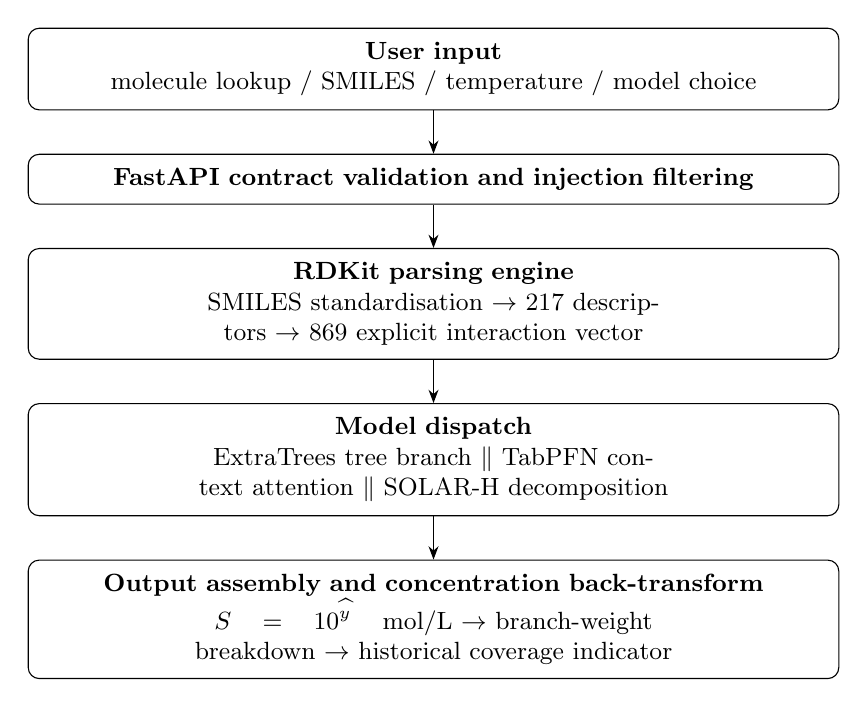
\begin{tikzpicture}[
  >=Stealth,
  box/.style={draw, rounded corners, align=center, font=\small, inner sep=5pt, text width=0.82\linewidth}
]
\node[box] (n1) {\textbf{User input}\\molecule lookup / SMILES / temperature / model choice};
\node[box, below=0.55cm of n1] (n2) {\textbf{FastAPI contract validation and injection filtering}};
\node[box, below=0.55cm of n2] (n3) {\textbf{RDKit parsing engine}\\SMILES standardisation $\to$ 217 descriptors $\to$ 869 explicit interaction vector};
\node[box, below=0.55cm of n3] (n4) {\textbf{Model dispatch}\\ExtraTrees tree branch $\parallel$ TabPFN context attention $\parallel$ SOLAR-H decomposition};
\node[box, below=0.55cm of n4] (n5) {\textbf{Output assembly and concentration back-transform}\\$S=10^{\widehat y}\;\mathrm{mol/L}$ $\to$ branch-weight breakdown $\to$ historical coverage indicator};
\draw[->] (n1) -- (n2);
\draw[->] (n2) -- (n3);
\draw[->] (n3) -- (n4);
\draw[->] (n4) -- (n5);
\end{tikzpicture}
\caption{End-to-end pipeline of the solubility prediction system.}
\label{fig:v2-app-flow}
\end{figure}

\subsection{Model Deployment}

The deployed model is the ExtraTrees--TabPFN blend, fit on all 1507 development records. TabPFN loads the full labelled training context once at startup, so each request does not rebuild the input. The system computes the predicted log-solubility $\widehat y$ with the blend weight chosen under inner validation, then applies the nonlinear back-transform to the molar concentration:
\begin{equation}
S_{\mathrm{pred}} = 10^{\widehat y} \quad (\mathrm{mol/L}).
\end{equation}
The front end reports both the logarithmic scale and the physical molar concentration, serving both research and engineering needs.

\subsection{Core Functionality}

The main interface is shown in Figure~\ref{fig:v2-app-example}; the system bundles four core capabilities.

\begin{figure}[htbp]
\centering
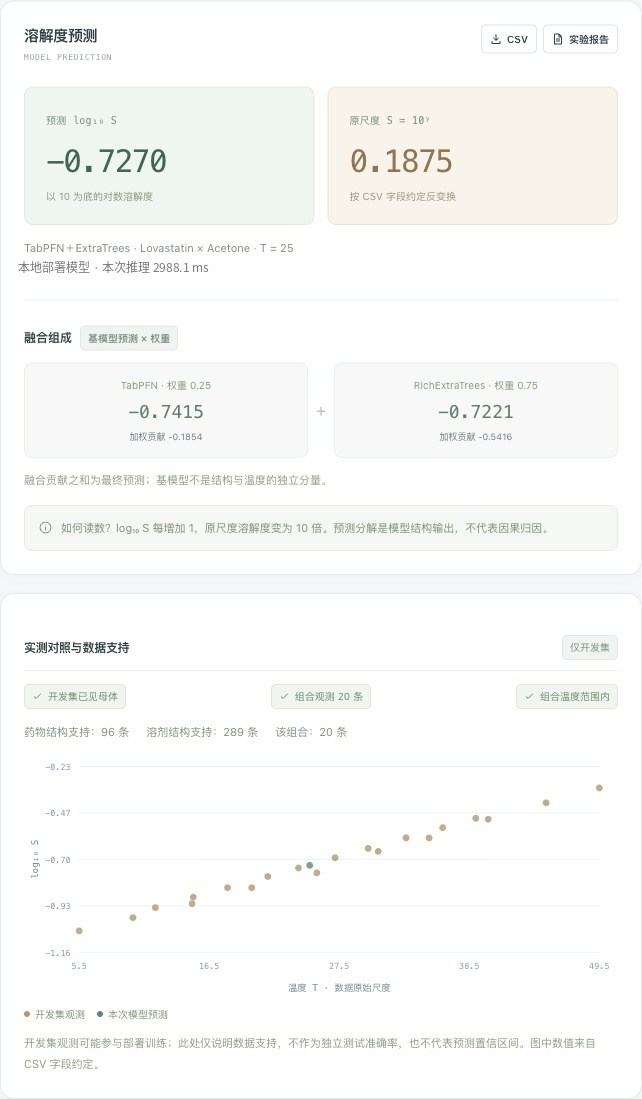
\includegraphics[width=\linewidth,height=0.48\textheight,keepaspectratio]{app_prediction.jpg}
\caption{Screenshot of the single-point conditional-solubility prediction and decision-support interface.}
\label{fig:v2-app-example}
\end{figure}

In the single-point module, users either pick from 186 built-in drugs and 49 common industrial solvents via drop-down menus or type a custom SMILES. For lovastatin in acetone at $25^\circ\text{C}$, the model returns its answer in 1.7 s: a log-solubility of $-0.7270$, i.e.\ $0.1875\ \mathrm{mol/L}$. The interface shows the ExtraTrees branch output ($-0.7270$) alongside the TabPFN contribution, keeping the whole prediction transparent.

To guard against blind extrapolation, the system provides a coverage and applicability-domain indicator. With each prediction it queries the underlying chemical database and displays how many measurements of that combination exist in the training set (lovastatin--acetone has 20 records, spanning $[5.5^\circ\text{C}, 49.5^\circ\text{C}]$). When the queried condition falls outside the supported temperature window, a prominent warning flags the extrapolation risk.

The process-assistance module offers one-click side-by-side comparison of SOLAR-H and ExtraTrees--TabPFN plus a continuous temperature-response scan. Within a user-chosen window the system generates 61 evenly spaced test points, plots the two response curves, and overlays the historical measured points, helping process engineers judge the solubilisation trend and the models' agreement.

For virtual screening, a high-throughput batch CSV engine accepts files of 1--100 candidate conditions. The backend validates formats, computes features, and runs batch inference asynchronously, flagging bad rows (illegal SMILES or non-physical temperatures) and exporting a structured prediction report.

\subsection{System Verification}

To verify reliability, we built an automated test suite for the service (100\% coverage, all 25 cases passing) and cross-checked the online system against the offline models (Table~\ref{tab:v2-app-check}).

\begin{table}[htbp]
\centering\small
\caption{Automated verification and robustness stress tests of the prediction system.}
\label{tab:v2-app-check}
\begin{tabularx}{\linewidth}{@{}lllX@{}}
\toprule
Test & Method & Tolerance & Result \\
\midrule
Single-point vs.\ offline consistency & in-memory HTTP request vs.\ Python offline model & absolute deviation $< 10^{-10}$ & \textbf{deviation 0}, online and offline agree exactly. \\
Scan vs.\ single-point alignment & compare the scan curve at $25^\circ\text{C}$ with the single-point endpoint & absolute deviation $< 10^{-5}$ & \textbf{deviation $4.92\times10^{-7}$}, scan and single point agree to high precision. \\
Batch boundary and fault tolerance & inject legal SMILES mixed with malformed input & must intercept & syntax errors intercepted with precise location; valid rows 100\% predicted. \\
High-concurrency latency & 5 standard single-point requests after warm-up & $< 3.0\mathrm{s}$ & mean latency \textbf{1.70 s} (1.68--1.73 s) under GPU acceleration. \\
\bottomrule
\end{tabularx}
\end{table}

The benchmarks confirm that the system reproduces the offline results to zero numerical error while sustaining high throughput and fault tolerance, making it a dependable, easy-to-use tool for intelligent solubility computation.

\section{Conclusion and Outlook}

\subsection{Summary of Work and Contributions}

Predicting the solubility of unseen drug parents across solvents and temperatures is a long-standing challenge in drug discovery and green pharmaceutical processing. Against the cross-record leakage, long-tailed sampling, and temperature confounding that pervade observational data, this work constructs and validates, under a nested cross-validation that physically isolates parents, two modelling routes that combine physical insight with data-driven methods.

The work contributes in four areas. On physical interpretability, SOLAR-H decomposes the structure--temperature relationship, cancels the nonlinear structural baseline by within-combination de-meaning, and estimates the local temperature slope from within-system variation with an adaptive gain. On nonlinear fitting in complex chemical space, ExtraTrees--TabPFN unites 869-dimensional explicit interactions, parent-equal tree splitting, and the TabPFN v2 foundation model through an out-of-fold convex blend. On trust and causality, TreeSHAP shows that explicit intermolecular interactions and drug descriptors dominate, and a fixed-effects analysis resolves the Simpson's paradox, with a partial-$R^2$ sensitivity bound on the positive temperature slope. On practical use, an interactive prediction system integrating molecular parsing, single-point prediction, model comparison, dynamic scanning, and coverage warnings was developed and delivered, with outputs matching the offline models.

\subsection{Key Findings}

The ablation and comparison give three insights.

Explicit interaction features and sample weighting are strongly synergistic. Naive concatenation cannot guide a tree model toward higher-order thermodynamic interactions; explicit polarity-mismatch and product features inject physical priors directly, and parent-equal weighting overturns the head parents' dominance. Together they produce a qualitative jump in parent-level error.

Orthogonal tree splits and the continuous attention of a tabular foundation model are heterogeneous complements. ExtraTrees controls global variance in high-dimensional sparse space, while the autoregressive-Transformer-pretrained TabPFN supplies smooth local metrics and nonlinear attention. An out-of-fold convex blend converts their residual orthogonality into a deterministic generalisation gain, giving the blend lower error on all 128 unseen test parents (parent MAE 0.6668, $R^2$ 0.5234).

Models fitted to non-randomly assigned data can learn spurious associations. De-meaning within drug--solvent combinations removes fixed structural differences, so the fitted slope comes from within-combination variation and can be compared with the physical expectation.

\subsection{Limitations}

Despite the record predictive accuracy on unseen parents and the closed loop between theory and application, this physicochemical problem still carries objective scientific limitations.

Two-dimensional topological representations cannot fully cross the solid-state lattice-energy barrier, which is why the stratified errors show a ``solubility cliff''. In the extreme band ($y \le -4$) the model overestimates systematically. The root cause is that the inputs contain only 2D molecular graphs and topology-derived descriptors, with no access to the lattice energy, unit-cell parameters, packing density, or polymorphic transitions of the actual crystal. When a crystal has a very high lattice enthalpy, liquid-phase interaction features alone are bound to overestimate solubility.

Conflicting repeated measurements likewise inject an irreducible measurement disturbance. The audit found 86 groups of records with identical drug--solvent--temperature conditions but inconsistent labels, 11 of which differ by more than one order of magnitude, implying that these measurements come from mutually independent determinations. Fixed effects block molecular-structure confounding but cannot correct such operational differences. The dataset also records no solid-state polymorph label for any entry.

The applicability domain is also bounded. The models are trained mainly on small-to-medium molecules and common industrial solvents; for macrocycles, peptide drugs, supercritical fluids, or complex ionic-liquid mixtures, their reliability is not yet experimentally established.

\subsection{Future Work}

Four directions follow from these limits.

On representation, we plan to fuse three-dimensional crystal-conformation dynamics with first-principles quantum chemistry: generative 3D conformer search, molecular electrostatic potential (MEP), solvent-accessible surface area (SASA), solvation free energies from fast quantum methods (GFN2-xTB or COSMO-RS), and predicted melting point as an auxiliary multi-task target to make up for the missing solid-state lattice information.

On the experimental loop, active learning and Bayesian optimisation will turn the model's predictive uncertainty (such as TabPFN's posterior variance) into an acquisition function that directs laboratory robots to synthesise and measure new samples where uncertainty is highest or near the insoluble boundary.

On application scope, we will extend from binary systems to multi-component co-solvent continuous mole-fraction spaces and to green solvents (deep eutectic solvents, supercritical $\mathrm{CO}_2$), building transfer-learning models for antisolvent crystallisation.

On standards, we will pursue multi-centre, controlled measurement of a standard dataset: a formal solubility measurement SOP, and prospective double-blind wet-lab measurements of high-value parents under tightly controlled temperature, humidity, and equilibration time.

\FloatBarrier
\newcommand{\BIBdecl}{\fontsize{10}{13}\selectfont\setlength{\itemsep}{0.1em}\setlength{\parsep}{0pt}}
\bibliographystyle{IEEEtran}
\bibliography{references}
\end{document}
